\section{Topologische Indizes} \label{sec:topologische_indizes}

Topologische Indizes sind mathematische Masse, die die topologische Struktur eines Graphen charakterisieren.
Sie können genutzt werden, um die Konnektivität oder Komplexität eines Netzwerks zu beschreiben, und sie haben zahlreiche Anwendungen in einer Vielzahl von Bereichen:
In der Chemie dienen topologische Indizes dazu, die Eigenschaften chemischer Verbindungen wie Siede-, Schmelzpunkte und Löslichkeit vorherzusagen.
Sie können auch verwendet werden, um die strukturellen und funktionellen Eigenschaften von Biomolekülen wie Proteinen und Nukleinsäuren zu untersuchen.
In der Biologie kann mithilfe von topologischen Indizes, um die Protein-Ligand-Bindungsaffinität vorhergesagt werden, was für das Arzneimitteldesign bedeutsam ist.
Topologische Indizes können auch zur Untersuchung der Struktur und Funktion biologischer Netzwerke eingesetzt werden, etwa Protein-Protein-Interaktionsnetzwerke und metabolische Netzwerke \cite[p.~199ff]{balaban_topological_1983}.
In sozialen Netzwerken können topologische Indizes verwendet werden, um die Struktur von Netzwerken zu analysieren und zu verstehen, wie sich Informationen durch diese verbreiten.

Der topologische Index ist ein numerischer Wert oder eine Sequenz für eine bestimmte diskutierte Struktur, die tatsächlich die physikalischen, chemischen und biologischen Eigenschaften eines Graphen abbildet \cite{manzoor_entropy_2020}.
Einige Indizes spiegeln die Grösse des Moleküls wider, z. B. der Kohlenstoffzahlindex, andere, z. B. der Balaban-Zentralindex, charakterisieren die Form \cite[p.~1]{rouvray_modeling_1987}.
\begin{theorem}[Topologischer Index]
    \label{thm:topologischer_index}%
    Ein topologischer Index ist eine numerische Invariante eines Graphen \cite[p.~235]{plavsic_harary_1993}.

    Topologische Indizes sind Zahlen, welche Graphen durch konstitutionelle Formeln aus mathematischen Operationen als numerische Werte repräsentieren. \cite[p.~16]{devillers_topological_2000}, \cite[p.~23]{devillers_topological_2000}.
\end{theorem}

\newpage
\subsection{Anwendung von topologischen Indizes}

Eine der Hauptanwendungen topologischer Indizes ist die Untersuchung der Eigenschaften chemischer Verbindungen, um diese basierend auf ihren strukturellen und funktionellen Eigenschaften zu klassifizieren. Topologische Indizes werden auch zugrunde gelegt, um die Struktur und Funktion von Biomolekülen wie Proteinen und Nukleinsäuren zu untersuchen \cite[p.~1015]{gonzalez-diaz_medicinal_2007}.
Topologische Indizes dienen auch dazu, wesentliche Einflussfaktoren zu identifizieren oder vorherzusagen, wie sich das Netzwerk im Laufe der Zeit verändern könnte \cite[p.~400]{watts_collective_1998}.

Topologische Indizes werden auch angewendet, um Probleme in anderen Bereichen wie Informatik, Ingenieurwesen und Wirtschaftswissenschaften zu lösen. So werden sie beispielsweise eingesetzt, um den kürzesten Weg zwischen zwei Punkten in einem Transportnetzwerk zu finden \cite{dijkstra_note_1959} und um die Ressourcenallokation in einer Lieferkette zu optimieren \cite{bazaraa_nonlinear_2013}.
Insgesamt liegt der Nutzen topologischer Indizes in ihrer Fähigkeit, ein quantitatives Mass für die topologische Struktur eines Graphen bereitzustellen, das zur Untersuchung der Eigenschaften komplexer Systeme und zur Lösung von Problemen in einer Vielzahl von Bereichen verwendet werden kann.

Topologische Indizes werden u. a. von Chemikern als Werkzeug zur Beschreibung chemischer Phänomene genutzt.
Die topologischen Indizes charakterisieren dabei sowohl die Grösse als auch die Form chemischer Spezies und spiegeln die Menge an Verzweigungen in Molekülen signifikant wider.
Chemiker sind somit in der Lage, das chemische Verhalten einer breiten Palette chemischer Substanzen in allen drei thermodynamischen Zuständen graphenbasiert genau zu modellieren \cite[p.~1]{rouvray_modeling_1987}.

Eine ihrer Eigenschaften, die als Einzigartigkeit oder Unterscheidungskraft bezeichnet wird, ist in der mathematischen Chemie und im strukturorientierten Arzneimitteldesign im Kontext der quantitativen Charakterisierung der Struktur von Molekülen ausführlich untersucht worden.
Im Allgemeinen erhält ein Index das Attribut degeneriert, wenn er für mehr als einen Graphen denselben Wert besitzt \cite[p.~1]{dehmer_information_2012}.

Weitere Wissenschaftler haben magnitudenbasierte Informationsindizes vorgeschlagen, um die Trennschärfe anderer klassischer topologischer Index für Alkanbäume und Isomere zu verbessern.
Alkanbäume sind zusammenhängende und azyklische Graphen, in denen der Grad eines Knotens höchstens 4 ist.
Zudem wird die Trennschärfe von informationstheoretischen Massen basierend auf Distanzen für chemische Graphen unterschieden, die einen Ring enthalten.
So ist die Einzigartigkeit verschiedener informationstheoretischer und nicht informationstheoretischer Massnahmen gegeben, indem polyzyklische Strukturen verwendet werden.
Als Ergebnis erweisen sich der Balaban-J-Index, die Summe der lokalen Vertex-Entropien und die magnitudenbasierten Informationsindizes als einzigartig, für diese Klasse von Graphen \cite[p.~1]{dehmer_information_2012}.

Neben empirischen Eigenschaften von Informationsmassen für Graphen – etwa das Bestimmen von Korrelationen zwischen den Massen – bestehen auch mathematische Probleme, z. B. der Nachweis verschiedener Ober- und Untergrenzen von Massnahmen.
Die Korrelationsfähigkeit zwischen zwei Graphmassen bezieht sich im Allgemeinen auf das Problem, ob sie strukturelle Informationen ähnlich erfassen.
Ausserdem wird die Klasse der Graphen-Entropiemasse, die durch Verwendung bestimmter Informationsfunktionale auf Grundlage der metrischen Eigenschaften von Graphen (z. B. der Nachbarschaft von Atomen) erhalten werden, verwendet, um Probleme in QSAR und QSPR zu lösen.
Insbesondere Dehmer et al. (2012) klassifizieren die sog. Mutagenität von Molekülen unter Verwendung dieser Massnahmen und unter Nutzung überwachter Lerntechniken \cite[p.~2]{dehmer_information_2012}.

Insgesamt werden in dieser Studie die Grenzen topologischer Indizes und Restriktionen bei deren Anwendung im grossen Massstab deutlich. Ein topologischer Index kann für eine bestimmte Graphenklasse eindeutig sein, aber er schlägt fehl, wenn das Mass auf eine andere Klasse angewendet wird \cite[p.~9]{dehmer_information_2012}.

Topologische Indizes \(TI(G)\) haben folgenden Anforderungen zu erfüllen:

\begin{lemma}[Topologische Indizes und Isomorphie]
    \label{thm:index_isomorphism}%
    Wenn \(G_1 \simeq G_2 \) (isomorph) sind, dann gilt \(TI(G_1) = TI(G_2)\).
    Im Umkehrschluss gilt bei \(TI(G_1) = TI(G_2)\), \( G_1 \simeq G_2\) nicht, da Indizes bei nicht isomorphen Graphen auch denselben Wert ergeben können.
\end{lemma}

Dieses Lemma wird in den zwei nachstehenden Beispielen verdeutlicht.

\begin{figure}[H]
    \begin{subfigure}{.4\textwidth}
        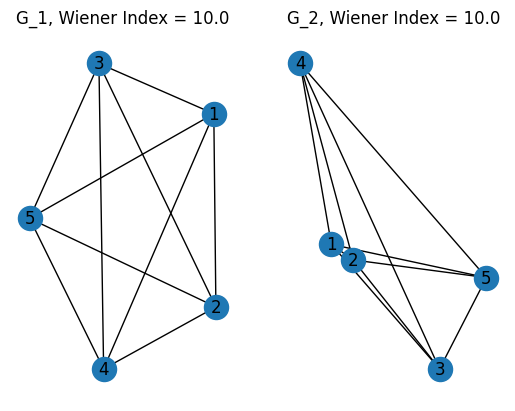
\includegraphics[width=\textwidth]{images/20_material_methods/lemma_2_proof_1.png}
        \label{fig:lemma_proof_1}
    \end{subfigure}%
    \hfill
    \vline
    \hfill
    \begin{subfigure}{.4\textwidth}
        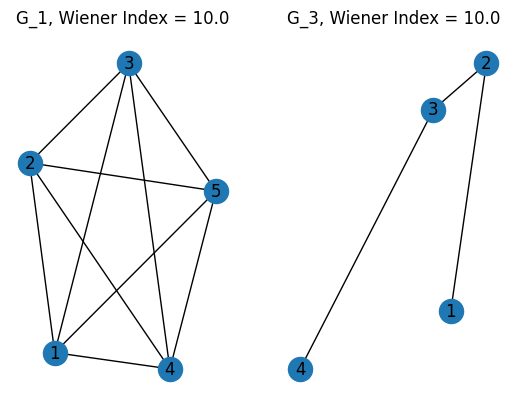
\includegraphics[width=\textwidth]{images/20_material_methods/lemma_2_proof_2.png}
        \label{fig:lemma_proof_2}
    \end{subfigure}
    \caption{Nachweis von Lemma \ref{thm:index_isomorphism}. G\_1 und G\_2 links, sind isomorphe Graphen. G\_1 und G\_3 in der rechten Abbildung sind nicht isomorphe Graphen, aber haben denselben Wiener Index.}
\end{figure}

Die topologischen Indizes können nach Balaban in verschiedene Kategorien eingeteilt werden \cite{balaban_1983_2014}.
Dabei spricht er von den folgenden Klassen: gradbasiert (Adjazenzmatrix), distanzbasiert (Distanz-Matrix), zentrische Indizes und informationstheoriebasiert.

\subsection{Gradbasiert}

Sei $\mathcal{G}$ ein molekularer Graph. Zwei Knoten von $\mathcal{G}$, die durch eine Kante verbunden sind, heissen \enquote{benachbart}.
Sind zwei Knoten $u$ und $v$ benachbart, besteht die Beziehung $u ~ v$.
Die Anzahl der Knoten von $\mathcal{G}$, die an einen gegebenen Knoten $v$ angrenzen, ist der \enquote{Grad} dieses Knotens und wird mit $dv(\mathcal{G})$ bezeichnet – wenn die Eindeutigkeit gegeben ist, mit $dv$.
Das Konzept des Grades in der Graphentheorie ist eng verwandt mit dem Konzept der Valenz in der Chemie \cite[p.~351]{gutman_degree-based_2013}.

\begin{figure}[H]
    \centering
    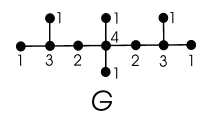
\includegraphics[width=0.3\textwidth]{images/20_material_methods/degree_graph.png}
    \caption{Graph $\mathcal{G}$ mit den Knotengeraden (Quelle: \cite[p.~351]{gutman_degree-based_2013})}
    \label{fig:degree_graph}
\end{figure}

Somit hat $\mathcal{G}$ sechs Knoten vom Grad $1$ (sogenannte \enquote{hängende} Knoten, die Methylgruppen darstellen) und zwei Knoten vom Grad 2 sowie zwei vom Grad 3 und einen Knoten vom Grad 4. Aus chemischen Gründen können die molekularen Graphen von Kohlenwasserstoffen keine Knoten besitzen, deren Grad grösser als 4 ist \cite[p.~351]{gutman_degree-based_2013}.

\subsubsection{Randić-Index}

Der Randić-Index und der Generalized Randić-Index sind Masse für die Struktur von Molekülen in der Chemie.
Der Randić-Index wurde von Milan Randić entwickelt und ist ein Mass für die \enquote{Heterogenität} oder die Unterschiedlichkeit der Atome in einem Molekül \cite{li_survey_2008}.

Er wird wie folgt berechnet:
\begin{equation}
    R = \sum_{uv \in E(G)}\frac{1}{\sqrt{d_u d_v}}
\end{equation}
Hierbei ist $d(i)$ die Anzahl der Nachbarn des Atoms $i$ und die Summe läuft über alle Atome des Moleküls.

Im Jahr 1998 haben Bollobás und Erdős den generalized Randić Index definiert, bei welchem auch die Anzahl der Bindungen zwischen den Atomen berücksichtigt wird \cite{li_survey_2008}.

Er wird folgendermassen berechnet:
\begin{equation}
    R_{\alpha}(G) = \sum_{uv \in E}{d(u) d(v)}^{\alpha}
\end{equation}
Im Allgemeinen wird der Generalized Randić-Index verwendet, wenn mehr Informationen über die Struktur eines Moleküls erlangt werden sollen, insbesondere über die Anzahl und Art der Bindungen zwischen den Atomen.
Der Randić Index hingegen ermöglicht nur Informationen über die Anzahl der Nachbarn eines Atoms und ist daher weniger detailliert.

Des Weiteren ist der $R_{\alpha}$ mit einem $\alpha = +1$ unter dem Namen \textit{Second Zagreb Index} definiert \cite{li_survey_2008}.

\subsubsection{Zagreb-Index}

Der erste Zagreb-Index wurde 1972 von Gutman und Trinajstic definiert \cite{xu_zagreb_2011}.
Er ist gleich der Summe der quadrierten Nachbarschaftsgrade aller Knoten.
\begin{equation}
    M_1(G) = \sum_{u \in V (G)} deg(v)^2
\end{equation}
Der zweite Zagreb-Index wird folgendermassen definiert:
\begin{equation}
    M_2(G) = \sum_{uv \in E (G)} deg(u) deg(v)
\end{equation}
Er ist die Summe der Produkte der Knotengrade von benachbarten Knoten \cite{das_zagreb_2015}.

\subsubsection{Harmonischer Index}

Der harmonische Index ist eine Variante des Randić-Index \cite[p.~562]{zhong_harmonic_2012}.
Er ist als die Summe der Gewichte aller Kanten von $uv$ von $G$ definiert, wobei $d(u)$ den Grad eines Knotens $u$ in $G$ abbildet.
Für einen Graphen $G$ lautet wird er wie berechnet \cite[p.~562]{zhong_harmonic_2012}:
\begin{equation}
    H(G) = \sum_{uv \in E (G)} \frac{2}{d(u) + d(v)}
\end{equation}
Die Berechnung des harmonischen Index kann aufwendig sein, insbesondere für grosse Graphen, aber es gibt Algorithmen und Techniken, um ihn effizient zu berechnen. 
Der harmonische Index hat auch interessante mathematische Eigenschaften und ist ein aktives Forschungsgebiet in der Graphentheorie \cite{li_harmonic_2014}.

\subsubsection{Atom-Bond Connectivity Index}

Dieser Index beschreibt die Verbindungen zwischen den Atomen einer Verbindung und berechnet den Index auf der Basis der Anzahl der Bindungen, die jedes Atom hat.
Die Verwendung von gradbasierten Metriken zur Charakterisierung von Verbindungen ist ein bedeutender Aspekt in der chemischen Informatik, und der Atom-Bond-Connectivity (ABC) Index ist eine gängige Methode zur Bewertung der Atomkonnektivität in Verbindungen \cite{estrada_atom-bond_1998}.

Die Formel zur Berechnung des ABC-Index lautet:
\begin{equation}
    ABC = \sum_{uv \in E(G)} \sqrt{\frac{d_u + d_v - 2} {d_u \times d_v}}
\end{equation}
Hierbei sind $d_u$ und $d_v$ die Grade der Knoten $u$ und $v$.

\subsection{Distanzbasiert}

\subsubsection{Wiener-Index}

Der Wiener-Index ist der erste topologische Index, der von Harold Wiener, einem Chemiker, eingeführt wurde \cite{fath-tabar_hyper-wiener_2011}.
Ein fundamentaler, distanzbasierter Index ist der Wiener-Index. Er ist als Summe der Abstände zwischen allen ungeordneten Scheitelpunktpaaren des Graphen definiert und heute aufgrund des breiten Anwendungsspektrums weitgehend verbreitet.
Insbesondere ist er einer der am häufigsten verwendeten topologischen Indizes in der mathematischen Chemie.
Angesichts dessen korreliert es stark mit vielen physikalischen und chemischen Eigenschaften molekularer Verbindungen, deren Eigenschaften nicht nur von ihrer chemischen Formel, sondern auch von ihrer molekularen Struktur abhängen \cite[p.~2]{cavaleri_group_2021}.
Es werden die Summen aller Abstände (kürzeste Wege) von jedem Knoten zu jedem anderen Knoten in die Berechnung einbezogen.
Der Wiener-Index ist definiert durch \cite[p.~17]{wiener_structural_1947}:
\begin{equation}
    W = \frac{1}{2}\sum^N_{i,j}d_{ij}
\end{equation}

\subsubsection{Hosoya-Index} \label{sec:hosoya_index}

Der Hosoya-Index, auch molekularer topologischer Index genannt, ist ein mathematisches Mass für die topologische Komplexität eines Moleküls.
Er ist definiert als die Summe der Quadrate des Grades jedes Scheitelpunkts im Molekulargraphen, wobei der Grad eines Scheitelpunkts die Anzahl der damit verbundenen Kanten ist.
Der Hosoya-Index korreliert nachweislich mit verschiedenen physikalischen und chemischen Eigenschaften von Molekülen wie Siedepunkt und Löslichkeit \cite[p.~397ff]{hosoya_topological_1972}.

Eine der frühesten wissenschaftlichen Arbeiten zum Hosoya-Index ist 1981 von F. Hosoya und Y. Tanaka in der Zeitschrift Chemical Physics Letters veröffentlicht worden.
In diesem Artikel stellen die Autoren das Konzept des Hosoya-Index vor und demonstrieren sein Potenzial als Mass für die molekulare Komplexität.
Seit seiner Einführung ist der Hosoya-Index auf dem Gebiet der chemischen und biochemischen Forschung weitverbreitet und Gegenstand zahlreicher wissenschaftlicher Arbeiten und Übersichtsartikel \cite[p.~397ff]{hosoya_topological_1972}.

Er wird folgendermassen berechnet \cite[p.~182]{hosoya_topological_1972}:
\begin{equation}
    Z = \sum_{k = 0}^{\lfloor N / 2 \rfloor} p(G, k)
\end{equation}
Dabei ist $ p(G, k) $ die Anzahl Möglichkeiten, in welcher $ k $ Knoten von $ G $ gewählt werden können, so dass keine zwei Knoten benachbart sind.
Das in den Gauss-Klammern stehende $ N / 2 $ ist die kleinste natürliche Zahl innerhalb $ N / 2 $.
Den grössten Hosoya-Index eines Graphen mit $ n $ Knoten erhält man von einem kompletten Graphen \ref{sec:complete}.

\subsubsection{Szeged-Index}

Der Szeged-Index ist ein Mass für den Informationsgehalt eines Graphen und wird verwendet, um die Komplexität oder Struktur des Graphen zu bewerten.
Er ist von Ivàn Gutman 1994 eingeführt worden und generalisiert das Konzept des Wiener-Index \cite{gutman_szeged_1998}.

Er lässt sich folgendermassen berechnen \cite[p.~2]{gutman_szeged_1998}:
\begin{equation}
    Sz(G) = \sum_{e \in E(G)} n_1(e | G)n_2 (e | G)
\end{equation}
Hier ist $ e $ eine Kante aus $ E $ im Graphen $ G $; $ e $ verbindet die Knoten $ u $ und $ v $, so wird auch $ e = uv $ oder $ e = vu $ geschrieben.
Für $ e = uv \in E(G) $ sei $ n_1(e | G) $ und $ n_2(e | G) $ die Anzahl Knoten von $G$, die näher zu Knoten $ u $ als Knoten $ v $ respektive für $n_2$ näher bei Knoten $ u $ als Knoten $ v $ sind \cite{gutman_szeged_1998}.

\subsection{Zentrische Indizes}

Die zentrischen Indizes wurden durch Balaban eingeführt und sind eine Gruppe von Indizes, die die zentrische Struktur eines Graphen beschreiben \cite{balaban_1983_2014}.
Sie verhalten sich ähnlich wie die Distanz-Indizes, da es bei der Suche nach dem zentralen Knoten auf die Distanz zwischen den Knoten ankommt.
Gemäss dem Jordanschen Zentrumssatzes ist der zentrische Knoten derjenige, der die geringste Summe der Distanzen zu allen anderen Knoten hat \cite[p.~32]{gross_graph_2018}. \\
Die Definition des Zentrums eines Graphens $ G $ ist eine Menge von Knoten $ V $, deren \textit{graph eccentricity} gleich dem Graph-Radius ist \cite[p.~35]{harary_graph_1994}.

\subsubsection{Balabans zentrischer Index B}

Der zentrische Index $B$ von Balaban wurde Entwickelt, um das Zentrum von Baumgraphen zu bestimmen \cite[p.~355]{balaban_chemical_1979}.
$ B $ wird ähnlich wie der erste Zagreb-Index aufgrund der quadratischen Formel definiert \cite[p.~355]{balaban_chemical_1979}.
\begin{equation}
    B = \sum_{i} \delta_i^2
\end{equation}

Dabei ist $ \delta_i $ die Anzahl Knoten, welche bei jedem Schritt $ i $ entfernt werden können, ohne dass der Graph zerfällt \cite[p.~355]{balaban_chemical_1979}.

\subsubsection{Estrada-Index}

Der Estrada-Index $ EE $ ist ein topologischer Index, welchen Estrada im Jahr 2005 eingeführt hat \cite{estrada_subgraph_2005}. 
Seinen Namen hat er jedoch erst 2007 von de la Peña \cite{de_la_pena_estimating_2007} erhalten. Er misst die Partizipation von allen Knoten in allen Teilgraphen eines Graphen \cite[p.~6]{estrada_subgraph_2005} und wird wie folgt berechnet \cite[p.~6]{estrada_subgraph_2005}:
\begin{equation}
    EE(G) = \sum_{i=1}^n e^{\lambda_i}
\end{equation}
Es ist $ G $ der Graph, $ n $ die Anzahl der Knoten und $ \lambda_i $ sind die Eigenwerte der Adjazenzmatrix $ A $.

\subsection{Informationstheoriebasiert}

Unter \enquote{Informationstheorie} wird ein Zweig der Mathematik verstanden, in dem die Quantifizierung und Analyse von Informationen thematisiert wird \cite[p.~82-83]{dehmer_information_2008}.
Informationstheoriebasierte Indizes stellen Masse dar, die Prinzipien der Informationstheorie verwenden, um den Informationsgehalt oder die Komplexität eines Systems quantitativ zu bewerten.
Ein Beispiel für einen auf der Informationstheorie basierenden Index ist die Entropie, die ein Mass für das Ausmass der Unsicherheit oder Zufälligkeit in einem System darstellt \cite[p.~767-768]{dehmer_information_2011}.
Entropie kann verwendet werden, um den Informationsgehalt einer Nachricht zu messen, indem bspw. das Ausmass der Unsicherheit quantifiziert und durch Erhalt der Nachricht reduziert wird \cite[p.~3]{iceland_multigroup_2004}.
Newman \cite[p.~2ff]{newman_structure_2003} diskutiert in diesem Kontext die Verwendung informationstheoretischer Indizes, einschliesslich der Entropie und gegenseitiger Informationen, um die Entwicklung von Informationen in komplexen Systemen zu untersuchen, die Zentralität von Knoten in Netzwerken zu quantifizieren sowie die Struktur und Funktion komplexer Netzwerke zu analysieren.

Balaban \cite[p.~16]{balaban_1983_2014} beschreibt zudem, dass laut einer Untersuchung die diversen informationstheoretischen Indizes eine tiefe diskriminierende Leistung aufweisen, was bedeutet, dass sie in der Lage sind, die Struktur eines Graphen zu unterscheiden, selbst wenn die Anzahl der Knoten und Kanten überaus gross ist. Eine Ausnahme ist der Balaban-J-Index.
Es ist später im Paper ein \emph{Super-Index} eingeführt worden, welcher ein Vektor ist, der aus den verschiedenen informationstheoretischen Indizes besteht \cite[p.~16]{balaban_1983_2014}. Dieser Super-Index besteht aus dem Informations-Orbit-Index $ I_{ORB}$, dem chromatischen Informationsindex $ I_{CHR} $, dem Graph-Distanz-basierten Informationsindex $ I^W_D $, dem Hosoya- und Randić-Informationsindex $ I_Z $ und $ I^E_X $ so wie dem orbitalen Informationsindex für Graphenverbindungen $ I_C $. \\
Im Rahmen dieser Arbeit wird jedoch nur der chromatische Informationsindex $ I_{CHR} $ untersucht.

\subsubsection{Chromatic Information Index}

Der Chromatic Information Index (CII) $ I_{CHR} $ ist ein Mass für den Informationsgehalt eines Graphen und wird verwendet, um die Komplexität oder Struktur des Graphen zu bewerten.
Er ist definiert als die Mindestanzahl von Farben, die erforderlich ist, um die Scheitelpunkte eines Diagramms richtig einzufärben, wobei Einschränkungen berücksichtigt werden,
die durch die Kanten zwischen den Scheitelpunkten vorgegeben werden. \\
Der CII ist ein nützliches Werkzeug zum Analysieren und Vergleichen der strukturellen Eigenschaften verschiedener Arten von Graphen und findet Anwendung in Bereichen wie Datenanalyse, Netzwerkwissenschaft und Informatik.
Er ist eng mit anderen Graphenfärbungsmassen wie der chromatischen Zahl, dem chromatischen Index und dem chromatischen Polynom verwandt \cite[p.~93ff]{bonchev_information_1985}.

Mowshowitz definiert den $ I_{CHR} $ als \textit{unique chromatic information content} (engl. für \enquote{einzigartiger chromatischer Informationsgehalt}) \cite[p.~13]{balaban_1983_2014}, welcher die chromatische Struktur eines Graphen repräsentiert \cite{mowshowitz_entropy_1968}.
\begin{equation}
    \hat{V} = \{ V_i \}^h_i=1(|V_i| = n_i(\hat{V}))
\end{equation}
Es ist $n$ die Anzahl der Knoten im Graphen $X$.
Es sei $\hat{V}$ die arbiträre chromatische Dekomposition von $X$, wo $h = \chi(X)$ gilt.
Dann sei $ I_{CHR}(X) $ der chromatische Informationsinhalt von $X$.
\begin{equation}
    I_{CHR}(X) = \min{V \{ -\sum_{i=1}{h}{\frac{n_i(V)}{n} \log \frac{n_i(V)}{n}} \} }
\end{equation}
